%%%% Dokumentklassen %%%%

\documentclass[a4paper,11pt,fleqn,dvipsnames,twoside,openany]{memoir} 	% Openright åbner kapitler på højresider (openany begge)

\usepackage{wrapfig}
%%%% PACKAGES %%%%
%% Oversættelse og tegnsætning %%
\usepackage[utf8]{inputenc}					% Input-indkodning af tegnsæt (UTF8)
\usepackage[danish]{babel}					% Dokumentets sprog
\usepackage[T1]{fontenc}					    % Output-indkodning af tegnsæt (T1)
\usepackage{ragged2e,anyfontsize}			% Justering af elementer
\usepackage{fixltx2e}						% Retter forskellige fejl i LaTeX-kernen
\usepackage{eso-pic}		
\newcommand\BackgroundPic{%
\put(0,0){%
\parbox[b][\paperheight]{\paperwidth}{%
\vfill
\centering
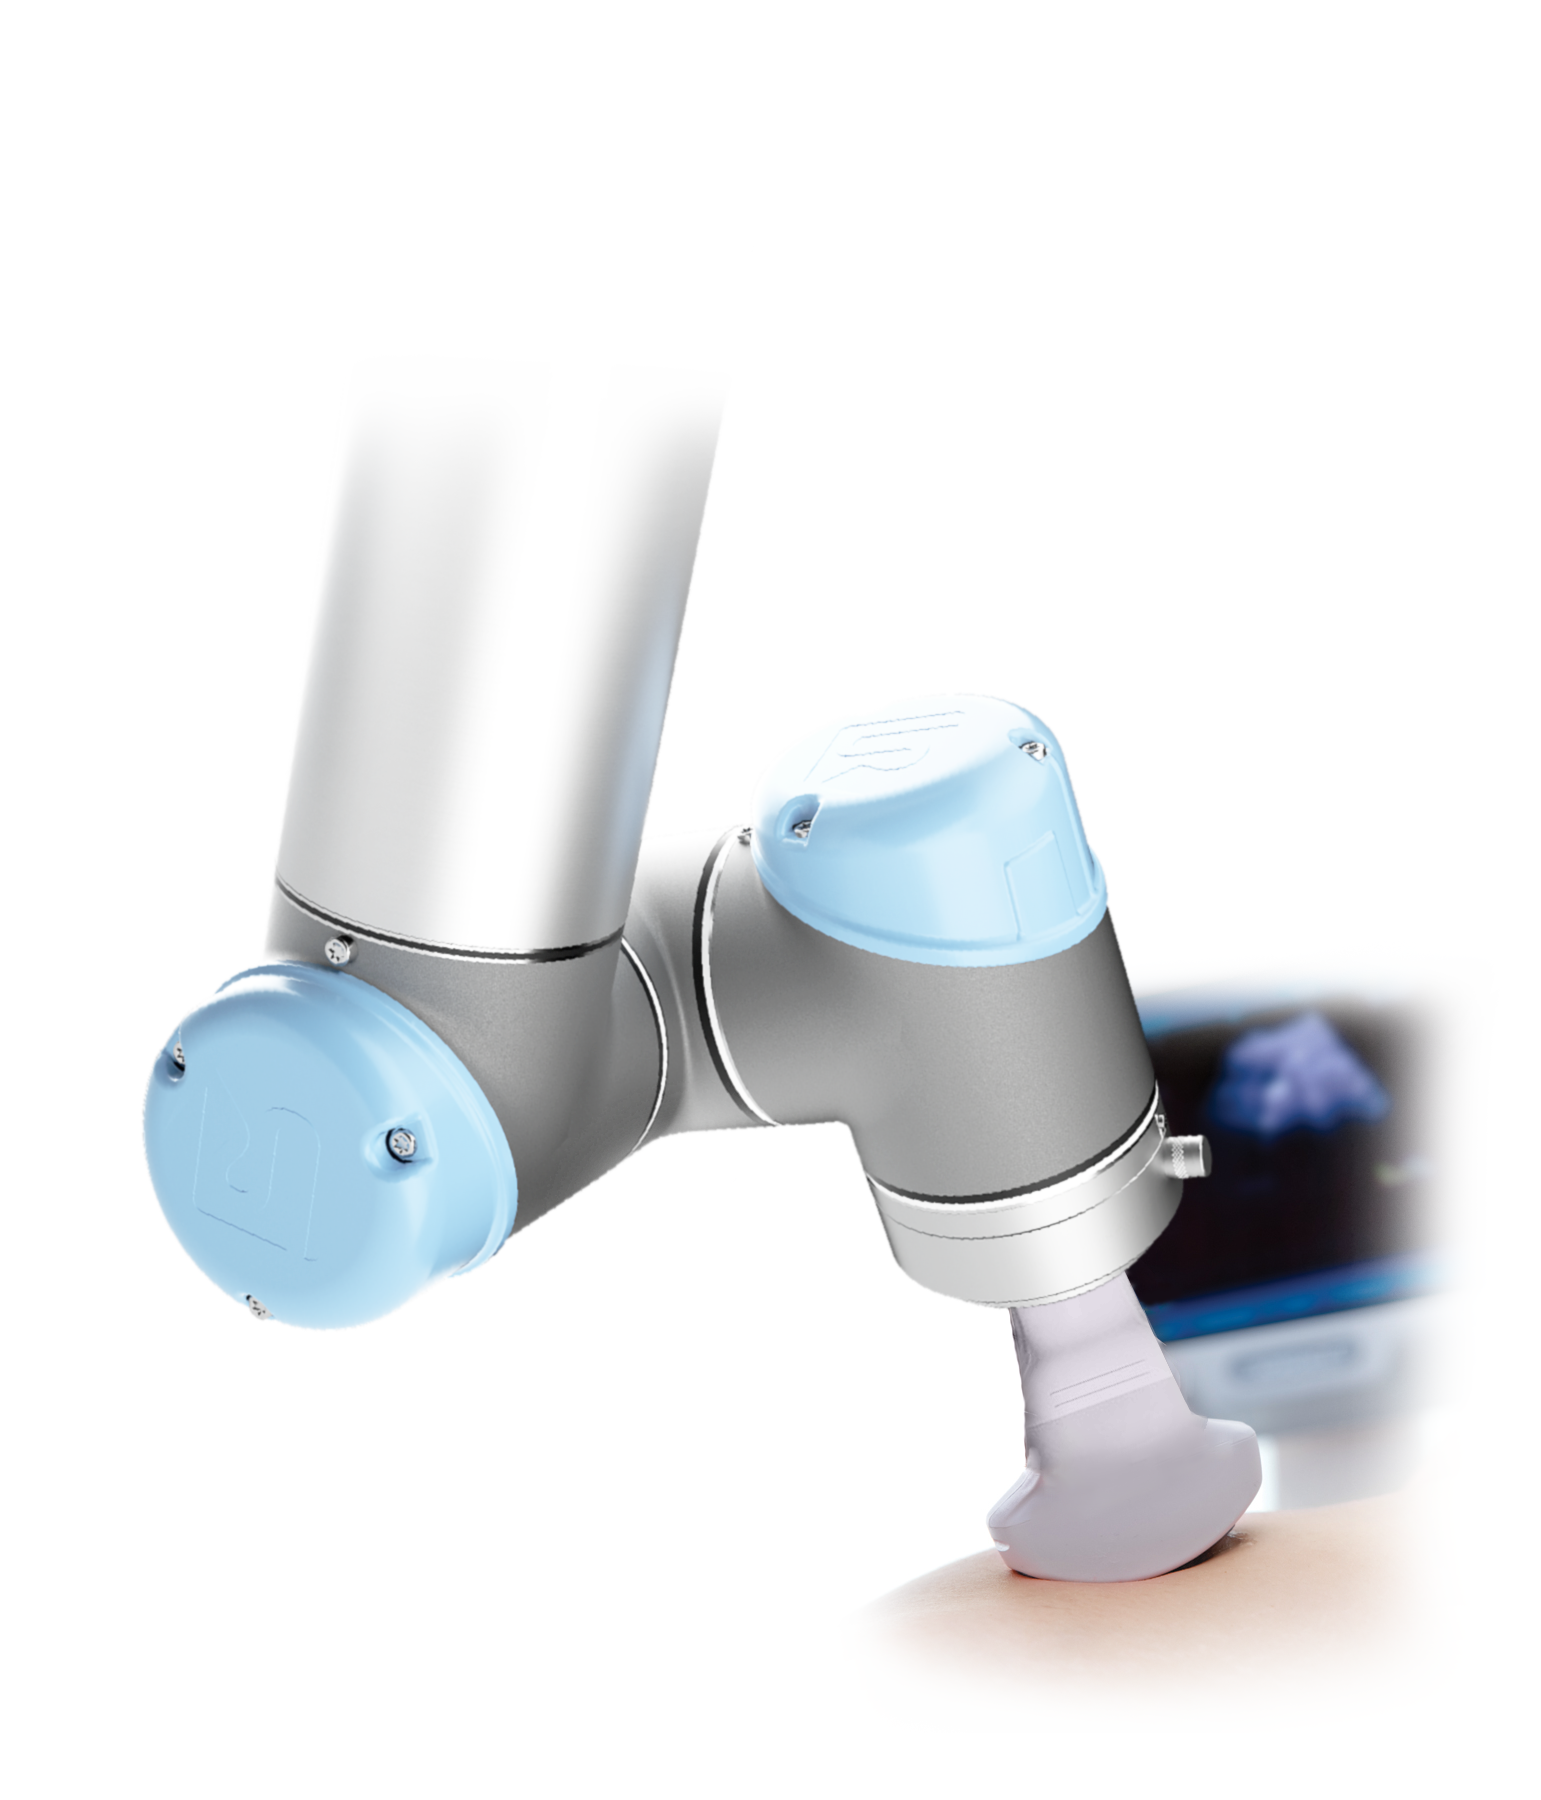
\includegraphics[width=\paperwidth,height=\paperheight,%
keepaspectratio]{figurer/forside.png}%
\vfill
}}}											
%% Figurer og tabeller (floats) %%
\usepackage{graphicx} 						% Håndtering af eksterne billeder (JPG, PNG, EPS, PDF)
\usepackage{multicol}         	            	% Muliggør output i spalter
\usepackage{rotating}						% Rotation af tekst med \begin{sideways}...\end{sideways}
\usepackage{xcolor}							% Definer farver med \definecolor. Se mere: http://en.wikibooks.org/wiki/LaTeX/Colors
\usepackage{flafter}						% Sørger for at floats ikke optræder i teksten før deres reference
\let\newfloat\relax 						% Justering mellem float-pakken og memoir
\usepackage{float}							% Muliggør eksakt placering af floats, f.eks. \begin{figure}[H]

%% Matematik mm. %%
\usepackage{amsmath,amssymb,stmaryrd} 		% Avancerede matematik-udvidelser
\usepackage{mathtools}						% Andre matematik- og tegnudvidelser
\usepackage{textcomp}                 		% Symbol-udvidelser (fx promille-tegn med \textperthousand)
\usepackage{rsphrase}						% Kemi-pakke til RS-saetninger, fx \rsphrase{R1}
\usepackage[version=3]{mhchem} 				% Kemi-pakke til flot og let notation af formler, f.eks. \ce{Fe2O3}
\usepackage{siunitx}						% Flot og konsistent præsentation af tal og enheder med \si{enhed} og \SI{tal}{enhed}
\sisetup{output-decimal-marker = {,}}		% Opsætning af \SI (DE for komma som decimalseparator) 
\usepackage{pdflscape}
\usepackage{afterpage}
%% Referencer og kilder %%
\usepackage[danish]{varioref}				% Muliggør bl.a. krydshenvisninger med sidetal (\vref)
\usepackage{natbib}							% Udvidelse med naturvidenskabelige citationsmodeller
\usepackage{xr}							    % Referencer til eksternt dokument med \externaldocument{<NAVN>}

%% Misc. %%
\usepackage{listings}						% Placer kildekode i dokumentet med \begin{lstlisting}...\end{lstlisting}
\usepackage{lipsum}							% Dummy text \lipsum[..]
\usepackage[shortlabels]{enumitem}			% Muliggør enkelt konfiguration af lister
\usepackage{pdfpages}						% Gør det muligt at inkludere pdf-dokumenter med kommandoen \includepdf[pages={x-y}]{fil.pdf}	
\pdfoptionpdfminorversion=6					% Muliggør inkludering af pdf-dokumenter, af version 1.6 og højere
\pretolerance=2500 							% Justering af afstand mellem ord (højt tal, mindre orddeling og mere luft mellem ord)	
\usepackage{hyperref}
%%%% CUSTOM SETTINGS %%%%
%% Marginer %%
\setlrmarginsandblock{3.5cm}{2.5cm}{*}		% \setlrmarginsandblock{Indbinding}{Kant}{Ratio}
\setulmarginsandblock{2.5cm}{3.0cm}{*}		% \setulmarginsandblock{Top}{Bund}{Ratio}
\checkandfixthelayout 						% Oversætter værdier til brug for andre pakker

%% Afsnitsformatering %%
\setlength{\parindent}{0mm}           		% Størrelse af indryk
\setlength{\parskip}{3mm}          			% Afstand mellem afsnit ved brug af double Enter
\linespread{1,1}							% Linjeafstand

%% Indholdsfortegnelse %%
\setsecnumdepth{subsection}		 			% Dybden af nummererede overskrifter (part/chapter/section/subsection)
\maxsecnumdepth{subsection}					% Dokumentklassens grænse for nummereringsdybde
\settocdepth{subsection} 					% Dybden af indholdsfortegnelsen
		
%% Opsætning af listings %%
\definecolor{commentGreen}{RGB}{34,139,24}
\definecolor{stringPurple}{RGB}{208,76,239}

\lstset{language=Matlab,					    % Sprog
	basicstyle=\ttfamily\scriptsize,		    % Opsætning af teksten
	keywords={for,if,while,else,elseif,		% Nøgleord at fremhæve
			  end,break,return,case,
			  switch,function},
	keywordstyle=\color{blue},				% Opsætning af nøgleord
	commentstyle=\color{commentGreen},		% Opsætning af kommentarer
	stringstyle=\color{stringPurple},		% Opsætning af strenge
	showstringspaces=false,					% Mellemrum i strenge enten vist eller blanke
	numbers=left, numberstyle=\tiny,		    % Linjenumre
	extendedchars=true, 					    % Tillader specielle karakterer
	columns=flexible,						% Kolonnejustering
	breaklines, breakatwhitespace=true,		% Bryd lange linjer
}

%% Navngivning %%
\addto\captionsdanish{
	\renewcommand\appendixname{Appendiks}
	\renewcommand\contentsname{Indholdsfortegnelse}	
	\renewcommand\appendixpagename{Appendiks}
	\renewcommand\appendixtocname{Appendiks}
	\renewcommand\cftchaptername{\chaptername~}		% Skriver "Kapitel" foran kapitlerne i indholdsfortegnelsen
	\renewcommand\cftappendixname{\appendixname~}	% Skriver "Appendiks" foran appendiks i indholdsfortegnelsen
}

%% Kapiteludssende %%
\definecolor{numbercolor}{gray}{0.7}		            % Definerer en farve til brug til kapiteludseende
\newif\ifchapternonum

\makechapterstyle{jenor}{					        % Definerer kapiteludseende frem til ...
  \renewcommand\beforechapskip{0pt}
  \renewcommand\printchaptername{}
  \renewcommand\printchapternum{}
  \renewcommand\printchapternonum{\chapternonumtrue}
  \renewcommand\chaptitlefont{\fontfamily{pbk}\fontseries{db}\fontshape{n}\fontsize{25}{35}\selectfont\raggedleft}
  \renewcommand\chapnumfont{\fontfamily{pbk}\fontseries{m}\fontshape{n}\fontsize{1in}{0in}\selectfont\color{numbercolor}}
  \renewcommand\printchaptertitle[1]{%
    \noindent
    \ifchapternonum
    \begin{tabularx}{\textwidth}{X}
    {\let\\\newline\chaptitlefont ##1\par} 
    \end{tabularx}
    \par\vskip-2.5mm\hrule
    \else
    \begin{tabularx}{\textwidth}{Xl}
    {\parbox[b]{\linewidth}{\chaptitlefont ##1}} & \raisebox{-15pt}{\chapnumfont \thechapter}
    \end{tabularx}
    \par\vskip2mm\hrule
    \fi
  }
}											        % ... her

\chapterstyle{jenor}						        % Valg af kapiteludseende - Google 'memoir chapter styles' for alternativer

%% Sidehoved %%

\makepagestyle{AAU}							        % Definerer sidehoved og sidefod udseende frem til ...
\makepsmarks{AAU}{%
	\createmark{chapter}{left}{shownumber}{}{. \ }
	\createmark{section}{right}{shownumber}{}{. \ }
	\createplainmark{toc}{both}{\contentsname}
	\createplainmark{lof}{both}{\listfigurename}
	\createplainmark{lot}{both}{\listtablename}
	\createplainmark{bib}{both}{\bibname}
	\createplainmark{index}{both}{\indexname}
	\createplainmark{glossary}{both}{\glossaryname}
}
\nouppercaseheads									% Ingen Caps ønskes

\makeevenhead{AAU}{\small BAC7 Automatisk Ultralydsscanner}{}{\leftmark}	% Definerer lige siders sidehoved (\makeevenhead{Navn}{Venstre}{Center}{Hoejre})
\makeoddhead{AAU}{\rightmark}{}{\small ASE}		            % Definerer ulige siders sidehoved (\makeoddhead{Navn}{Venstre}{Center}{Højre})
\makeevenfoot{AAU}{\small \thepage}{}{}						% Definerer lige siders sidefod (\makeevenfoot{Navn}{Venstre}{Center}{Højre})
\makeoddfoot{AAU}{}{}{\small \thepage}						% Definerer ulige siders sidefod (\makeoddfoot{Navn}{Venstre}{Center}{Højre})

\copypagestyle{AAUchap}{AAU}							% Sidehoved for kapitelsider defineres som standardsider, men med blank sidehoved
\makeoddhead{AAUchap}{}{}{}
\makeevenhead{AAUchap}{}{}{}
\makeheadrule{AAUchap}{\textwidth}{0pt}
\aliaspagestyle{chapter}{AAUchap}					% Den ny style vælges til at gælde for chapters
													% ... her
															
\pagestyle{AAU}										% Valg af sidehoved og sidefod


%%%% CUSTOM COMMANDS %%%%

%% Billede hack %%
\newcommand{\figur}[4]{
		\begin{figure}[H] \centering
			\includegraphics[width=#1\textwidth]{billeder/#2}
			\caption{#3}\label{#4}
		\end{figure} 
}

%% Specielle tegn %%
\newcommand{\decC}{^{\circ}\text{C}}
\newcommand{\dec}{^{\circ}}
\newcommand{\m}{\cdot}


%%%% ORDDELING %%%%

\hyphenation{mmHg}    %% Her kan defineres ordelingen for specifikke ord med "-". De forskellige ord adskilles med mellemrum. Fx \hyphenation{er-hvervs-liv-et Himmelstrup ka-kao}. I de fleste tilfælde kan LaTeX selv stå for det.

%%%% Tilføjelser af min preample %%%%

% Booktabs:
% The booktabs package is needed for better looking tables. 
\usepackage{booktabs}

% Caption:
% For better looking captions. See caption documentation on how to change the format of the captions.
\usepackage[hang, font={small, it}]{caption}

% Hyperref:
% This package makes all references within your document clickable. By default, these references will become boxed and colored. This is turned back to normal with the \hypersetup command below.
\usepackage{hyperref}
	\hypersetup{colorlinks=false,pdfborder=0 0 0}

% Cleveref:
% This package automatically detects the type of reference (equation, table, etc.) when the \cref{} command is used. It then adds a word in front of the reference, i.e. Fig. in front of a reference to a figure. With the \crefname{}{}{} command, these words may be changed.
\usepackage{cleveref}
	\crefname{equation}{formel}{formler}
	\crefname{figure}{figur}{figurer}	
	\crefname{table}{tabel}{tabeller}
	\crefname{section}{afsnit}{afsnit}
	\crefname{chapter}{kapitel}{kapitler}

% Mine tilføjelser:
\usepackage{nameref}                      %% Bruges til at kunne referere til kapitler og afsnits navne.
\usepackage{units}                        %% Bruges til at gøre fx 1/2 samlet med: \nicefrac{1}{2}.
\usepackage{tabu, longtable}              %% Bruges til tabeller.
\setlength{\tabulinesep}{2ex}             %% Definerer linjeafstand i tabeller.
\usepackage{enumerate}                    %% Bruges til lister.
\usepackage{tabto}                        %% Giver mulighed for TAB med fx \tabto{3em}.
\usepackage[hyphenbreaks]{breakurl}       %% Bruges til websiders url'er.
\renewcommand{\UrlFont}{                  %% Definerer url-font.
\small\ttfamily}                          %
\bibliographystyle{plain}                 %% Definere bibliografien. Ses til sidst i dokumentet i kapitlet Litteratur.
\usepackage[explicit]{titlesec}
\usepackage{longtable,tabu}
\usepackage{longtable}
\usepackage{todonotes}
\presetkeys{todonotes}{inline}{}
\externaldocument{Accepttest}

\titlespacing\section{0pt}{12pt plus 4pt minus 2pt}{0pt plus 2pt minus 2pt}
\titlespacing\subsection{0pt}{12pt plus 4pt minus 2pt}{0pt plus 2pt minus 2pt}
\titlespacing\subsubsection{0pt}{12pt plus 4pt minus 2pt}{0pt plus 2pt minus 2pt}
\raggedbottom

\begin{document}
\begin{titlingpage}
\begin{center}

~ \\[3cm]


\includegraphics[width=0.6\textwidth]{figurer/ASE}~\\[1cm]

\textsc{\LARGE Aarhus School of Engineering}\\[1.5cm]

\textsc{\Large Sundhedsteknologi og Informations- og kommunikationsteknologi}\\

\textsc{\Large Bachelorprojekt}\\[0.5cm]

\textsc{\Large Automatisk Ultralydsscanner} \\[1cm]

\noindent\makebox[\linewidth]{\rule{\textwidth}{0.4pt}}\\
[0.5cm]{\Huge Sætningsliste}
\noindent\makebox[\linewidth]{\rule{\textwidth}{0.4pt}}

\end{center}

Charlotte Søgaard Kristensen (201371015) \newline
Mathias Siig Nørregaard  (201270810)\newline		 
Marie Kirkegaard (201370526) \newline  


\textit{Vejleder} \newline
Associate Professor\\
Michael Alrøe\\
Aarhus School of Engineering


\vfill

\begin{center}
{\large \today}
\end{center}

\end{titlingpage}

\tableofcontents

\chapter{Forkortelser}
Dette dokument indeholder liste over forkortelser og forklaringer til projektets dokumenter. 

\section{Forkortelser til dokumentation}
Nedenfor er en tabel, med alle de forkortelser der er blevet brugt i projektets dokumenter. 

\begin{table}[htb]
\begin{tabular}{ | m{6em} | m{30em} | } \hline

\textbf{Forkortelse} & \textbf{Forklaring} \\ \hline
BDD & Block Definition Diagram \\\hline
CSK & Charlotte Søgaard Kristensen \\ \hline 
DTO & Data Transfer Objekter \\\hline
FURPS+ & Funkctionality, Usability, Reliability, Performance, Supportability and Ekstra \\\hline
GUI & Graphical User Interface, Grafisk brugergrænseflade \\ \hline 
IBD & Internal Block Diagram \\\hline
IKT & Informtions- og kommunkationsteknologi\\\hline
MDD & Medical Device Direktive \\\hline
MK &  Marie Kirkegaard \\ \hline
MoSCoW & Must, Should, Could and Would \\\hline
MSN & Mathias Siig Nørregaard \\ \hline 
ST & Sundhedsteknologi \\\hline
SysML &  System Modeling Language \\\hline
TCP & Tool Center Point \\\hline
TCP/IP & Transmission Control Protocol/IP-protokollen \\\hline
UC & Use Case \\\hline
UML & Unified Modeling Language\\\hline
\end{tabular}
\caption{Forkortelser}
\end{table}
\newpage

\section{Forkortelser til Medicinsk Godkendelse}
\begin{table}[htb]
\begin{tabular}{ | m{6em} | m{30em} | } \hline

\textbf{Forkortelse} & \textbf{Forklaring} \\ \hline
EMC & Elektromagnetisk kompatibilitet \\ \hline
ESD & Elektrostatiske sensitive enheder  \\ \hline
FMECA & Failure Mode, Effects og Criticality Analysis \\ \hline
GUI & Grafiskbrugergrænseflade \\ \hline 
MDD & Medical Device Directive 93/42/EØF \\ \hline 
PMS & Post market surveillance \\ \hline 
QMS & Kvalitetsstyringssystem \\ \hline 
63204:2006 & DS/EN 63204:2006 - Software for medicinsk udstyr - Livscyklusprocesser for software \\ \hline 
ISO 13485:2012 & DS/EN ISO 13485:2012 - Medicinsk udstyr – Kvalitetsledelsessystemer – Krav til lovmæssige formål \\ \hline 
ISO 14971:2012 & DS/EN ISO 14971 – medicinsk udstyr – Anvendelse af risikoledelse i forbindelse med medicinsk udstyr. \\ \hline
\end{tabular}
\caption{Forkortelser til medicinsk godkendelse}
\end{table}

\chapter{Forklaringer} 
Nedenfor findes der forklaringen på de tegn, opstillinger og standardindstillinger, som der er blevet anvendt i projektet.

\section{Forklaringer på tegn}
\begin{table}[htb]
\begin{tabular}{ | m{6em} | m{30em} | } \hline

\textbf{Tegn} & \textbf{Forklaring} \\ \hline
[  ] & Tekst markeret med [  ] betyder at det er en knap \\ \hline 
\end{tabular}
\caption{Forklaringer}
\end{table}

\section{Forklaring på forsøgsopstilling}
Detaljeret forsøgsopstilling til accepttesten. 

\begin{itemize}
\item \textbf{Robotarm er tilsluttet:} Sæt Universal Robots' UR10 strømkabel til en stikkontakt og tryk på dens 'On/Off' knap i højre øverste hjørne af skærmrammen. Tilslut et ethernetkabel af typen RJ45 fra Robotarm til access point. Sæt access points strømkabel til en stikkontakt. På computeren forbindes der på WiFi til 'opentele'.
\item \textbf{3D kamera er tilsluttet:} Sæt Microsoft Kinect 2.0s strømkabel til en stikkontakt. Sæt Microsoft Kinect 2.0s USB-kabel i computerens USB 3.0 port.
\item \textbf{PC Appliaktion er startet:} Gennemførsel af samtlige tests i tabel \ref{uc1_test_h_label} i dokumentet Accepttest
\item \textbf{Ultralydsscanner er tændt:} Gøres ved at trykker på start-knappen på ultralydsscanneren
\item \textbf{Robotarm står i Ikke-standard positur:} Sæt Universal Robots' UR10 strømkabel til en stikkontakt og tryk på dens [On/Off] knap i højre øverste hjørne af skærmrammen. Når den har bootet færdig tryk på 'Go to initialization screen' på UR10s touchskærm. Tryk på [On]. Tryk på [START]. Tryk på [OK] i højre nederste hjørne. Tryk på [Play]-knappen nederst på skærmen. Tryk på fanen [Move] øverst på skærmen. Tryk på [Feature]-dropdownen, og vælg [Base]. Tryk på en af tekstboksene i [TCP]-rammen. Indtast de koordinater der findes i posituren 'Ikke-standard Positur'. Tryk på [OK]. Hold [Auto] nede indtil 'Auto' bliver greyed out. Tryk [OK]. Tryk på [On/Off]-knappen i højre øverste hjørne af skærmrammen. Tryk på [Shutdown Robot] på touchskærmen.
\item \textbf{Testobjekt er placeret inden for afgrænsning} Gøres ved, at Testobjektet ligger inden for bordet under 3D kamera. 
\end{itemize}


\section{Robotarm positurer}
En positur er en definition for den position og rotation som Robotarm kan have. Til accepttesten er der defineret nogle positurer til at tjekke at softwaren virker som den skal. 

\begin{itemize}
\item \textbf{Standard Positur:} Er angivet ved disse koordinater:
\begin{itemize}
\item Position X: $-$ 160 mm
\item Position Y: $-$ 268 mm
\item Position Z: $+$ 500 mm
\item Rotation X: $+$ 1.09 radianer
\item Rotation Y: $+$ 1.7 radianer
\item Rotation Z: $-$ 1.9 radianer
\end{itemize}

\item \textbf{Ikke-standard Positur:} Er angivet ved disse koordinater:
\begin{itemize}
\item Position X: $-$ 130.00 mm
\item Position Y: $-$ 250.00 mm
\item Position Z: $+$ 900.00 mm
\item Rotation X: $+$ 0.8 radianer
\item Rotation Y: $+$ 1.5 radianer
\item Rotation Z: $-$ 1.7 radianer
\end{itemize}

\item \textbf{3D Scan Positur:} Er angivet ved disse koordinater:
\begin{itemize}
\item Position X: $-$ 100.00 mm
\item Position Y: $-$ 650.00 mm
\item Position Z: $+$ 600.00 mm
\item Rotation X: $+$ 3.1416 radianer
\item Rotation Y: $\pm$ 0 radianer
\item Rotation Z: $+$ 3.1416 radianer
\end{itemize}
\end{itemize}

\end{document}